% LaTeX template for a short report (written for MSES scenario modelling)
% uses LaTeX documentclass "article" for use of sections (not chapter) and References (not Bibliography)
% for Chapters and Bibliography use "documentclass "report
\documentclass[10pt]{article}   % Use article class with 10pt letter
%\documentclass[10pt]{report}
\usepackage[utf8]{inputenc}

%\usepackage[T1]{fontenc}  % 8-bit encoding, helps hyphenation of accented characters -
% https://tex.stackexchange.com/a/677/42066

% Use A4 paper and set margins:
%\usepackage[a4paper, twoside, top=2.0cm, left=3.0cm, bottom=2.0cm, right=2.0cm]{geometry}
\usepackage[a4paper, twoside, top=2.0cm, left=2.0cm, bottom=2.0cm, right=2.0cm]{geometry}
%\usepackage[a4paper, top=2.5cm, left=2.5cm, bottom=2.5cm, right=2.5cm]{geometry}

\usepackage[english]{babel}  % Hyphenation and more for English

\usepackage{pgf}      % Include graphics inside figures using \pgfimage
\usepackage[font=small, labelfont=bf]{caption}  % Stylize figure, table, etc. captions

\usepackage{parskip}         % Replace paragraph indentations with white lines
\usepackage[hyphens]{url}    % Take care of urls, e.g. wrapping in the Bibliography (hyphens: also break at -)

\usepackage{xspace}   % \xspace saves the user from having to type \  or {} after a macro name in text.

% Use the appendix package for nicer appendices:
%\usepackage[toc,page]{appendix}  % MvdS
\usepackage[titletoc]{appendix}
%\usepackage[toc,page,title]{appendix}  % Use \begin{appendices} ... \end{} iso \appendix

% \usepackage[numbib,numindex]{tocbibind}  % Add ToC, List of Figures/Tables/Code listings, Bibliography and Index to ToC
% \usepackage[]{tocbibind}       % Add ToC, List of Figures/Tables/Code listings, Bibliography and Index to ToC
\usepackage[nottoc]{tocbibind}   % ToC without extra "Contents" entry...

\usepackage{amsmath,amssymb,bbm}
\usepackage{enumerate}         % Choose alternative numberings, e.g. \begin{enumerate}[a.]

\usepackage{listings}          % Code listings
\usepackage[section, above, below]{placeins}  % \FloatBarrier - flush floats before \section by default
% \usepackage{pgf}               % Figures

\usepackage{color}
\definecolor{lightgrey}{rgb}{0.9,0.9,0.9}
\definecolor{darkgreen}{rgb}{0.0,0.6,0.0}

% Citations:

% option1: use natbib/bibtex with MvdS_number_url.bst
%\usepackage[numbers, square]{natbib}  % Use numbered citations with square brackets
%\bibliographystyle{MvdS_number_url}  % Use [1], print url = field  (plain doesn't print urls)

%option2: use biblatex/biber without *.bst file
\usepackage[backend=biber, style=numeric, citestyle=numeric-comp, sorting=none]{biblatex} 
\setlength\bibitemsep{0.5\baselineskip}
\usepackage{csquotes}

% \bibliography{mybibliography} % old-style for backward comp. in preamble for biblatex/bibtex
\addbibresource{mybibliography.bib}  % new syntax for BibLaTeX


\usepackage{fancybox}  % Use \ovalbox for key strokes

\newcommand{\ldf}{\usefont{OT1}{cmr}{m}{n}}     % Select default LaTeX font - Computer Modern Roman
%\newcommand{\ldf}{\usefont{OT1}{cmss}{m}{n}}     % Select default LaTeX font - Computer Modern Sans
%\newcommand{\ldf}{\usefont{OT1}{phv}{m}{n}}     % Select default LaTeX font - Helvetica
\newcommand{\ttbf}{\usefont{OT1}{lmtt}{bx}{n}}  % Select bold typewriter font

%\usepackage[font=sf]{caption}  % Use sans-serif font for float captions - not exactly Helvetica



\newcommand{\note}[1]{\color{red}\textbf{#1}\color{black}\xspace}
\newcommand{\marc}[1]{\color{red}\textbf{Marc: #1}\color{black}\xspace}

\newcommand{\myChapter}[1]{
  \chapter{#1}
  \minitoc  % Create a ToC of this chapter
}


% General expressions:
\newcommand{\eg}{\emph{e.g.}\xspace}
\newcommand{\ie}{\emph{i.e.}\xspace}
\newcommand{\etc}{\emph{et cetera}\xspace}
\newcommand{\ff}{\emph{ff}\xspace}

% CLI symbols:
\newcommand{\pipe}{$|$}      % Needed to avoid | in \index{}
\newcommand{\logor}{$|\,|$}  % Needed to avoid | in \index{}
\newcommand{\home}{\url{~}}  % Home directory


% Often used code names:
\newcommand{\NULL}{\code{NULL}}
\newcommand{\void}{\code{void}}
\newcommand{\stdout}{\code{stdout}}
\newcommand{\stderr}{\code{stderr}}

% Man pages:
\newcommand{\man}[2]{\texttt{man #1 #2}\xspace}
\newcommand{\mancmd}[1]{\texttt{man #1}\xspace}

% Code:
\newcommand{\prototype}[3]{\hspace*{2em}\texttt{#1} {\ttbf #2\ldf}(\texttt{#3});\xspace}  % function prototype
\newcommand{\var}[2]{\hspace*{2em}\texttt{#1} {\ttbf #2\ldf};\xspace}  % variable declaration
\newcommand{\code}[1]{\texttt{#1}\xspace}  % inline code
\newcommand{\codeb}[1]{\ttbf #1\ldf\xspace}  % inline bold code
\newcommand{\codeline}[1]{\hspace*{2em}\texttt{#1}}  % separate code line

\newcommand{\cli}[1]{\noindent\hspace*{2em}\code{\$ #1}}  % command line input
\newcommand{\clir}[1]{\noindent\hspace*{2em}\code{\# #1}}  % command line input root
\newcommand{\clo}[1]{\noindent\hspace*{2em}\code{#1}}  % command line output
\newcommand{\clitem}[1]{\item[\code{\$}] \code{#1}}  % cli in itemized list, with $ as bullet
\newcommand{\clitemb}[1]{\item[\codeb{\$}] \codeb{#1}}  % cli in itemized list, with $ as bullet - bold

\newcommand{\key}[1]{\Ovalbox{\texttt{#1}}\xspace}  % key press/combination
\newcommand{\keyb}[1]{\Ovalbox{\ttbf #1\ldf}\xspace}  % key press/combination bold


% Heat pumps
\newcommand{\COP}{\mathrm{COP}}  % COP in "math mode"
\newcommand{\COPh}{\COP_{\mathrm{heating}}}  % COP_heating in "math mode"

\newcommand{\Qh}{Q_{\mathrm{H}}}
\newcommand{\Qc}{Q_{\mathrm{C}}}
\newcommand{\Th}{T_{\mathrm{H}}}
\newcommand{\Tc}{T_{\mathrm{C}}}

\newcommand{\Tin}{T_{\mathrm{in}}}
\newcommand{\Tout}{T_{\mathrm{out}}}

\newcommand{\Ph}{P_{\mathrm{heat}}}
\newcommand{\Pheat}{P_{\mathrm{heat}}}
\newcommand{\Pc}{P_{\mathrm{cool}}}
\newcommand{\Pcool}{P_{\mathrm{cool}}}
\newcommand{\Pel}{P_{\mathrm{el}}}

\newcommand{\degr}{^\circ}
\newcommand{\tdeg}{$\degr$\xspace}
\newcommand{\degC}{\degr\mathrm{C}}
\newcommand{\tdegC}{$\degC$\xspace}

  % Custom commands

\usepackage[pdftex]{hyperref}
\hypersetup{
  colorlinks = true,  % They get a red box around them if false, better set colour to black?
  linkcolor = blue,
  filecolor = magenta,
  citecolor = blue,
  urlcolor = blue,
  % linkcolor = black,
  % citecolor = black,
  % urlcolor = black,
  pdftitle = House Model References,
  pdfauthor = Trung Nguyen,
  pdfsubject = House Models,
  pdfkeywords = house - models - Python,
  pdfcreator = TeXStudio pdfLaTeX2 on Windows,
  pdfproducer = TeXStudio pdfLaTeX2 on Windows,
  bookmarksnumbered = true,  % Number sections in PDF toc
}

\usepackage[onehalfspacing]{setspace}
\usepackage{float}

\usepackage{graphicx}
\usepackage{multirow}

%\renewcommand{\thesection}{\arabic{section}}  % needed for documentclass "report" with sections





% Title page:
\title{The PID Python Control Libraries}
\author{Trung Nguyen\\
HAN University of Applied Sciences\\
Arnhem, The Netherlands} %\\

\begin{document}
	
\ldf  % Set LaTeX default font

% Set up code listing style:
\lstset{
	language=Python,
	% Fonts:
	basicstyle=\ttfamily\footnotesize,
	%keywordstyle=\ttfamily,
	%identifierstyle=,
	%commentstyle=\ttfamily\scriptsize,
	% B/W code:
	% commentstyle=\ttfamily\itshape,  % Italic
	% stringstyle=\ttfamily,
	% identifierstyle=\ttbf,           % Bold typewriter type
	% keywordstyle=\ttbf,              % Bold tt
	% Colour:
	commentstyle=\scriptsize\ttfamily\color{brown},
	stringstyle=\ttfamily\color{darkgreen},
	identifierstyle=\color{blue},
	keywordstyle=\ttfamily\color{red},
	% Spaces:
	showstringspaces=false,
	breaklines=true,
	breakatwhitespace=true,
	% Line numbering:
	numbers=left,
	numberstyle=\tiny,
	stepnumber=2, 
	numbersep=5pt,
	% Frames:
	frame=single,
	frameround=tttt,
	backgroundcolor=\color{lightgrey},
	morekeywords={pthread\_create},
}

%\renewcommand{\thelstlisting}{\thechapter.\arabic{lstlisting}}  % This is the default?
%\numberwithin{lstlisting}{section}  % AMSmath: number code listings per section
%\numberwithin{lstlisting}{chapter}  % AMSmath: number code listings per chapter

\maketitle

%\begin{center}
%	\today
%\end{center}

\tableofcontents

\newpage

% \chapter{Introduction}

\section{Introduction}

The report give an overview and compare between the available  PID and advance python control packages. The different PID forms will be discussed in section 2. In section 3 and 4 are the most used PID python packages in practice with their advantages and disadvantages. Finally section 5 give an overview on some advance control and optimization python library.


\newpage

\section{The PID Forms}
% \subsection{The PID Forms}

The PID controller are available on 3 main different form: Interactive, Non interactive (“standard”, “mixed” or sometimes “ideal) and Parallel.  

\textbf{The series form} sometime also call classical, real or interactive in equation (1) is the oldest controller used for direct field control which is either both of its input (PV) and output (MV) are directly connected to field or process equipment \cite{Wolfgang}. The original pneumatic and electronic controllers had this algorithm, and it is still found in many digital PID controllers today. The controller has been programmed to implement the interacting PID equation even though it is no longer an artifact of the hardware. The rationale for this programming is to have the digital controller behave identically to the legacy analog electronic or pneumatic controller it is replacing. This way, the proven tuning parameters of the old controller may be plugged into the new digital controller, yielding the same results.  
The famous Ziegler-Nichols PID tuning method was developed for this controller algorithm. 

\begin{figure}[H]
	\centering
	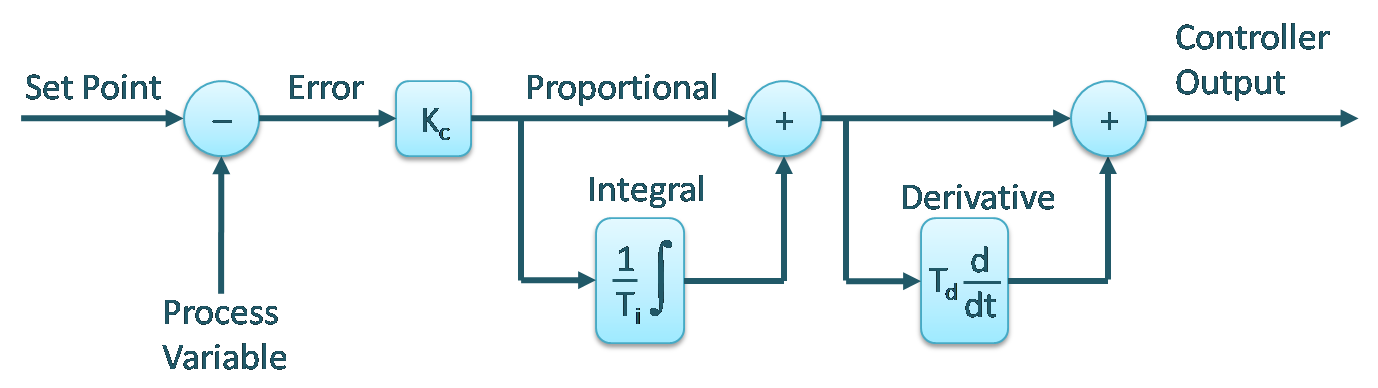
\includegraphics[width=0.8\columnwidth]{Pictures/series.png}
	\caption[Short title]{Serial form PID Controller \cite{PID}}
	\label{figure: Serial PID}
\end{figure}

\begin{equation}
\label{eqn:1}
    CO = K_c\cdot\left(e + \frac{1}{T_i}\int e\cdot dt \right)\cdot \left(1 + T_d\frac{de}{dt} \right)
\end{equation}


% A third version, with origins in the peculiarities of pneumatic controller mechanisms and analog electronic circuits, is called the Series or Interacting equation: 

% This “interacting” equation is an artifact of certain pneumatic and electronic controller designs. p Back when these were the dominant technologies, and PID controllers were modular designed such that integral and derivative actions were separate hardware modules included in a controller at additional cost beyond proportional-only action, the easiest way to implement the integral and derivative actions was in a way that just happened to have an interactive effect on controller gain. In other words, this odd equation form was a sort of compromise made for the purpose of simplifying the physical design of the controller. 

\textbf{The Ideal form} or non interactive algorithm is also called the standard or ISA algorithm. This form of controller is the classical teaching model of PID algorithms. It gives a clear understanding of P, I and D control, since: P-control, I-control and D-control can be seen independently of each other. Then, PID is effectively a combination of independent P, I and D-control actions. This can be seen in figure \ref{figure: Ideal PID} and euqation (2).
Since P, I and D algorithms are calculated independently in an ideal PID-controller. The Cohen-Coon and Lambda PID tuning rules were designed for this algorithm

\begin{figure}[H]
	\centering
	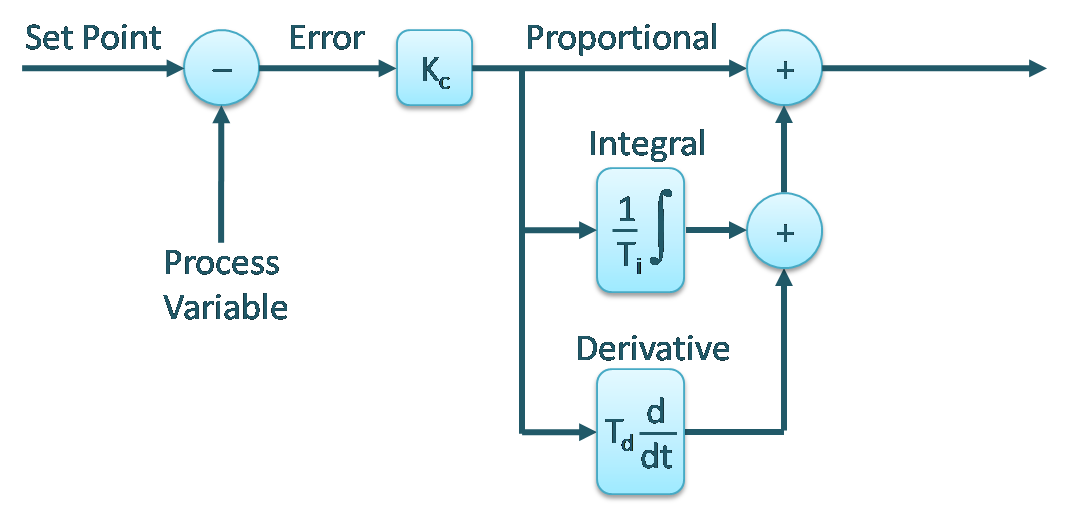
\includegraphics[width=0.8\columnwidth]{Pictures/ideal.png}
	\caption[Short title]{Ideal form PID Controller \cite{PID}}
	\label{figure: Ideal PID}
\end{figure}

\begin{equation}
\label{eqn:2}
    CO = K_c\cdot\left(e + \frac{1}{T_i}\int e\cdot dt +T_d\frac{de}{dt} \right)
\end{equation}

% An ideal process variable is a noise-free, refined and optimized variable. They are a result
% of computer optimization, process modeling, statistical filtering and value prediction
% algorithms

Note: If no derivative is used (i.e. Td = 0), the interactive and non interactive controller algorithms are identical. 

\textbf{The parallel form} has not often discussed in academic textbooks, but it is widely used nowadays in the  industry sector (distributes control system (DCSs) and PLCs application). This algorithm is simple to understand, but more difficult to tune. It has no controller gain affecting all three control modes (3 controller-action need to be tune separately), as a result it take more time to get the correct controller parameters. 

% Adjusting the proportional gain should be supplemented by adjusting the integral and derivative settings at the same time.

\begin{figure}[H]
	\centering
	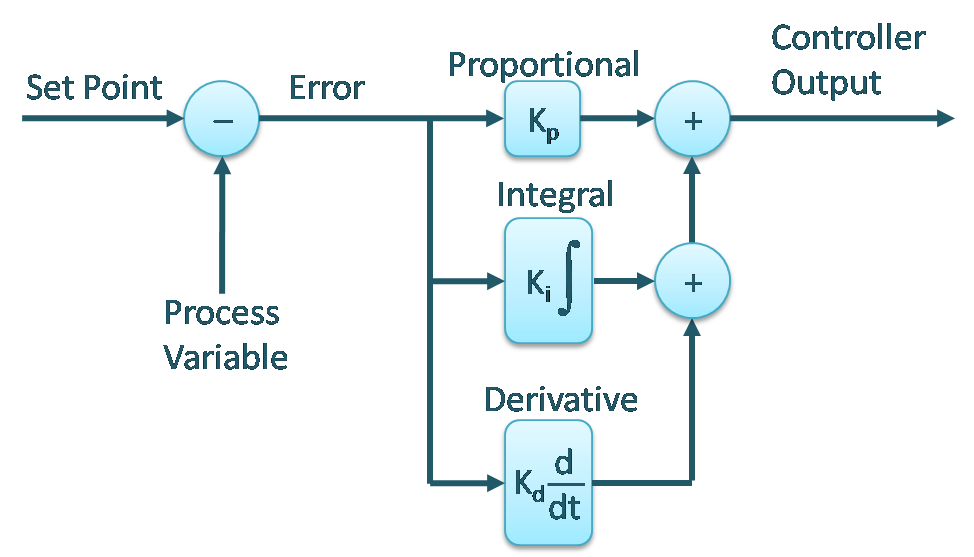
\includegraphics[width=0.8\columnwidth]{Pictures/parallel.png}
	\caption[Short title]{Parallel form PID Controller \cite{PID}}
	\label{figure: Parallel PID}
\end{figure}

\begin{equation}
\label{eqn:3}
    CO = K_p\cdot e + K_i\int e\cdot dt +K_d\cdot\frac{de}{dt}
\end{equation}

\textbf{Significance of Different Algorithms }

The biggest difference between the controller algorithms is that the parallel controller has a true proportional gain ($K_p$), while the other two algorithms have a controller Gain ($K_c$). The  $K_c$ Gain affects all three modes (Proportional, Integral and Derivative) of the Series and Ideal controllers, while $K_p$  affects only the proportional mode of a Parallel controller. 

This difference has a major impact on the tuning of the controllers. All the popular tuning rules (Ziegler-Nichols, Cohen-Coon, Lambda, and others) assume the controller does not have a parallel structure. 

% To tune a Parallel controller using any of these rules, the Integral time has to be divided and derivative time multiplied by the calculated Controller Gain. 

The second difference between the controller algorithms is the interaction between the \textbf{Integral} and \textbf{Derivative} modes of the Series (Interactive) controller. This is only of significance if the Derivative mode is used. In most PID controller applications, Derivative mode is not used  In practice D-action is not often used because of its sensitivity to the sensor noise. 

% Beyond the differences mentioned above, controllers also differ in the way the changes on controller output is calculated (positional and velocity algorithms), in the way Proportional and Derivative modes act on set point changes, in the way the Derivative mode is limited/filtered, as well as a interesting array of other minor differences. These differences are normally subtle, and should not affect your tuning. 

% To cut a long story short, it is hard to prescribe a particular form to implement a PID controller, each has its drawbacks and advantages. The standard structure is the most widespread in the field of industry. 
In the end, when tuning the controller, it is important to know what structure of the controller is (There are formulas to switch from one to another).


\newpage

\section{PID in practice.}
% Implement PID in practice
The Ideal and parallel PID in equation (1) and (2) can be easily converted from one to another with  $K_i = \frac{Kc}{T_i}$ and $K_d = \frac{Kc}{T_d}$.

Let Consider the independent PID equation (parallel):
\begin{equation}
\label{eqn:4}
     CO = K_p\cdot e + K_i\int e\cdot dt +K_d\cdot\frac{de}{dt}
\end{equation}

Where CO is the controller output, e=SP-PV, SP is the setpoint, PV the process variable (system output). Differentiating both sides of [4] gives:

\begin{equation}
\label{eqn:5}
    dCO = K_p\cdot de + K_i\cdot e \cdot dt + K_d\frac{d(de)}{dt}
\end{equation}

Using difference to approximate the differential we get discrete PID equation.

\begin{equation}
\label{eqn:6}
    CO(t) = CO(t-1) + K_p[e(t) - e(t-1)] + K_i\cdot T \cdot e(t) + \frac{K_d}{T}[e(t) - 2e(t)-1) + e(t-2)]
\end{equation}

Where T is the sampling period. The D-term of this equation contains set point and changes in set point may cause an unwanted change in CO (a Dirac function \cite{Delta_Function}, some time call derivative Kick ). Remove set point from D-term we get equation [6] (e = SP - PV, de = dSP -dPV, when SP is constant de = dPV).

\begin{equation}
\label{eqn:7}
    CO(t) = CO(t-1) + K_p[e(t) - e(t-1)] + K_i\cdot T \cdot e(t) + \frac{K_d}{T}[PV(t) - 2PV(t)-1) + PV(t-2)]
\end{equation}

Many industrial PID controllers use equation [6] (e.g. Allen Bradley PLCs). However, if we remove set point from both P-term and D-term, we get a still better PID equation [7].

\begin{equation}
\label{eqn:8}
    CO(t) = CO(t-1) + K_p[PV(t) - PV(t-1)] + K_i\cdot T \cdot e(t) + \frac{K_d}{T}[PV(t) - 2PV(t)-1) + PV(t-2)]
\end{equation}

To implement PID controller in practice a few more things need to be addressed.

\begin{itemize}
    \item Windup protection.
    \item On the fly tuning: a good PID controller allow changing the parameters when the process is running.
    \item Online Controller Switching or bumpless transfer:  allow smooth transition from one type of controller to another (ex: switch from PID to manual control, or MPC).
    \item 2 DOF (degree of freedom) PID (Optional) 
\end{itemize}

A good explanation on the practical problems and solution can be found in the the blog series improving the Beginner’s PID by Brettbeauregard \cite{Improving_PID}.


\newpage

\section{The PID Python Libraries}

Most of PID python libraries had been developed base on the Arduino PID and series blog by Beauregard \cite{Arduino_PID}  \cite{Improving_PID}. The Arduino version has been updated by 
Gelraen \cite{Arduino_PID_V2} on January 2021.

\subsection{Python packages.}
% \textbf{}
This subsection will give a quick overview on the most use python packages.

\textbf{Simple PID} \cite{Simple_Pid} follow the guideline implementation by Brett Beauregard  \cite{Improving_PID}. The package has included the windup protection, the derivative kick avoidance, online parameters tuning, smooth controller transition from Auto (PID on) to manual. The last update was on 17 November 2020

\textbf{ivPID} \cite{ivPID} PID controller implementation base on equation [\ref{eqn:4}] with windup protection. This package does not has derivative kick avoidance or smooth controller switching.

\textbf{DvG${\_}$PID${\_}$Controller} \cite{DvG_PID_Controller}: another Arduino library \cite{Arduino_PID} ported to Python by Dennis van Gils (a senior research of Twente University) in july 2020. This package has include all functionality from Arduino library ( windup protection, derivative kick, controller switch, bumpless transfer).

\subsection{PID design example with Jupiter notebook}

There are many other PID controller example had been written in python. A few more example are mentioned below:

An explanation on PID controller and python implementation can be found in \href{https://apmonitor.com/pdc/index.php/Main/ProportionalIntegralDerivative}{apmonitor dynamic and control website}.

\begin{figure}[H]
	\centering
	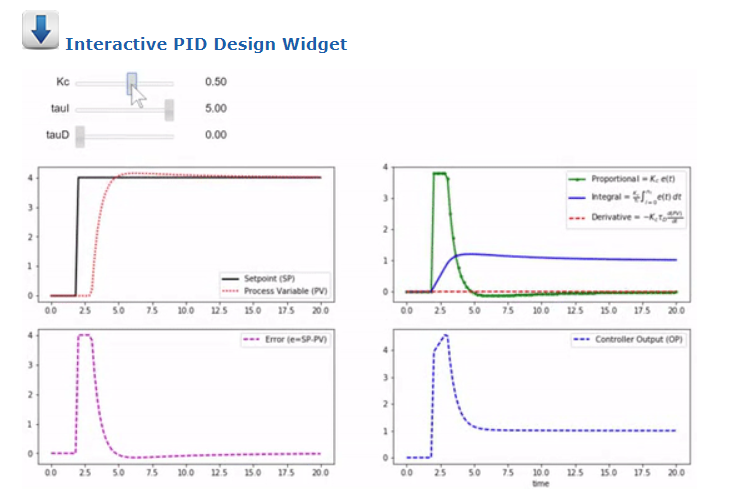
\includegraphics[width=0.8\columnwidth]{Pictures/PID_interactive.png}
	\caption[Short title]{Pid interactive notebook on apmonitor}
	\label{figure:interactive notebook}
\end{figure}

\newpage

A Jupyter/Python notebooks series on PID controller on (chapter 4) chemical process course of Notre Dame University\cite{CBE}.

\begin{figure}[H]
	\centering
	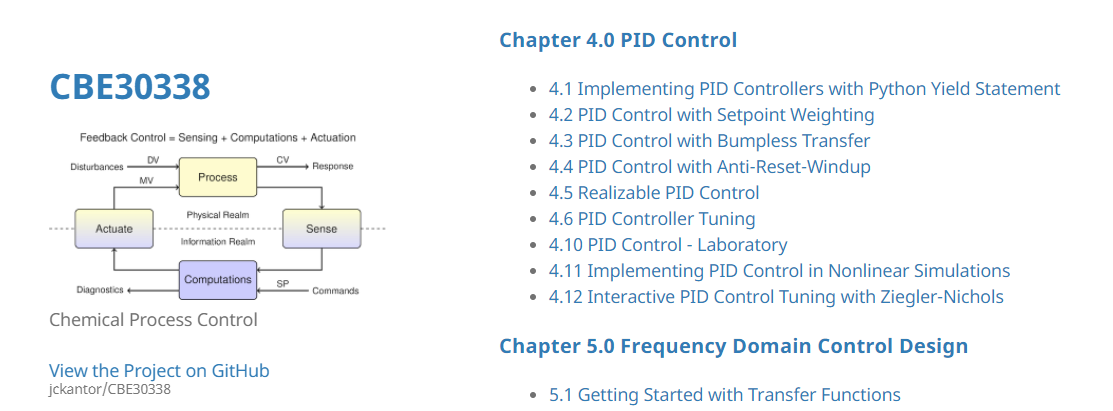
\includegraphics[width=0.8\columnwidth]{Pictures/PID_NotreDame.png}
	\caption[Short title]{Pid controller notebook series of Notre Dame University chemical process course.}
	\label{figure:NotreDame notebook}
\end{figure}

\newpage
\section{Python control system packages.}

In this chapter some advance python control and optimization packages will be discussed.

The first one is \textbf{python Control Systems} Library v0.84 \cite{Control_Lib} \cite{GitControl_Lib} with the last update on 16/03/2021 (the day when this report is written).

The main features are: 

\begin{itemize}
    \item Linear input/output systems in state-space and frequency domain

    \item Nonlinear input/output system modeling, simulation, and analysis

    \item Block diagram algebra: serial, parallel, and feedback interconnections

    \item Time response: initial, step, impulse

    \item Frequency response: Bode and Nyquist plots

    \item Control analysis: stability, reachability, observability, stability margins

    \item Control design: eigenvalue placement, LQR, H2, Hinf, MPC

    \item Model reduction: balanced realizations, Hankel singular values

    \item Estimator design: linear quadratic estimator (Kalman filter)
    
    \item The optimal control module with optimization based controllers for nonlinear systems with state and input constraints.

\end{itemize}

Another python package for machine learning and optimization is \textbf{GEKKO Optimization Suite}\cite{gekko2018}. It is coupled with large-scale solvers for linear, quadratic, nonlinear, and mixed integer programming (LP, QP, NLP, MILP, MINLP). Modes of operation include parameter regression, data reconciliation, real-time optimization, dynamic simulation, and nonlinear predictive control. The paper release with the package has been selected as a 2020 Best Paper by the journal Processes (figure: \ref{figure:Gekko}). 

\begin{figure}[H]
	\centering
	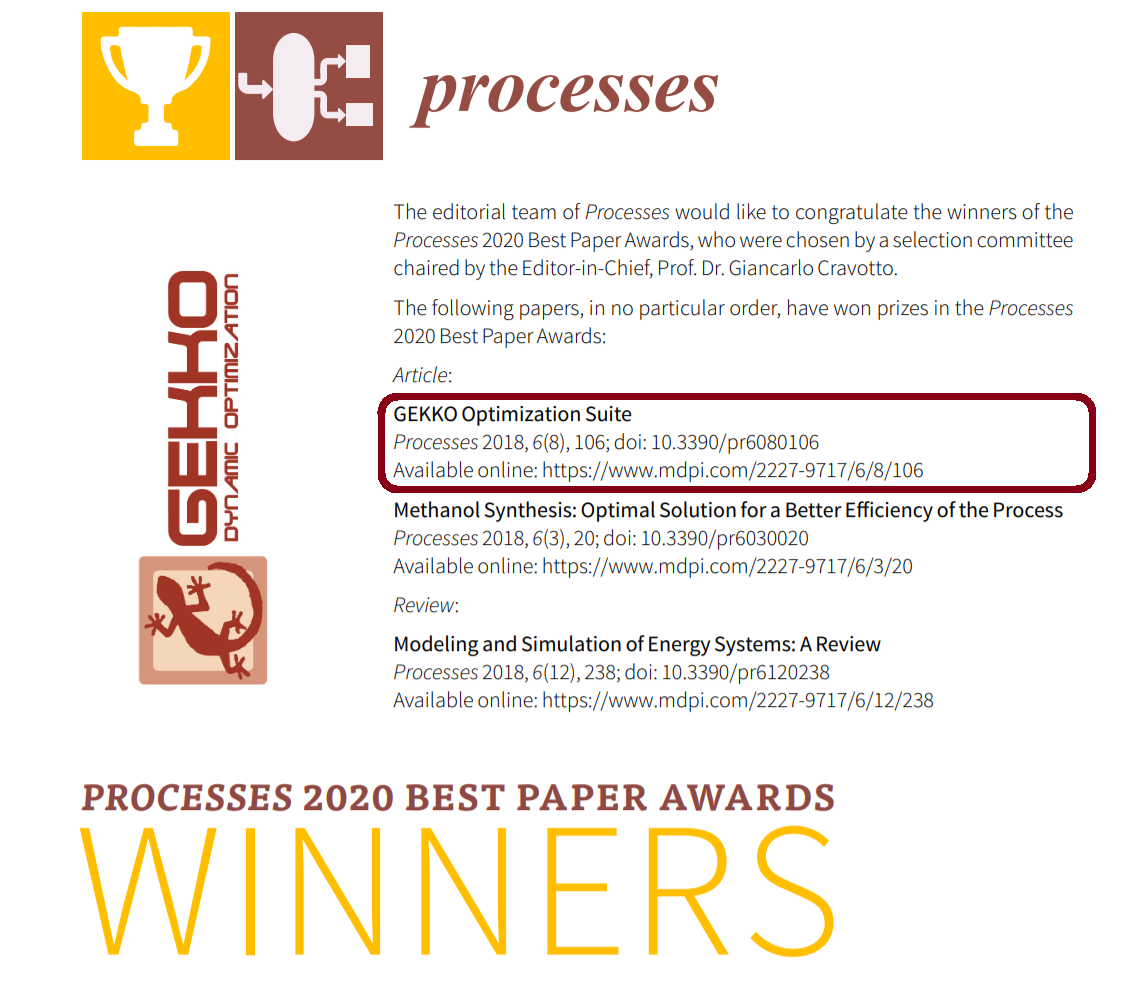
\includegraphics[width=0.8\columnwidth]{Pictures/gekko_best_paper2020.png}
	\caption[Short title]{Gekko best paper award 2020}
	\label{figure:Gekko}
\end{figure}

 Beside the 2 python packages which have been mentioned above there is a collection of Jupiter python/notebook series on optimization and control CBE 30338 (figure \ref{figure:CBE}) and CBE 32338 (\ref{figure:CBE_Lab}) Chemical Process Control \cite{CBE} \cite{CBE_Lab}. The notebooks series contain a lot of python example on optimization technique. For example, the linear programming has been mentioned in section 6.3 \cite{CBE} CBE 30338 (\ref{figure:CBE}) and the model predictive control in section 5.1, 5.2 \cite{CBE_Lab} CBE 32338 (\ref{figure:CBE_Lab}) 

\begin{figure}[H]
	\centering
	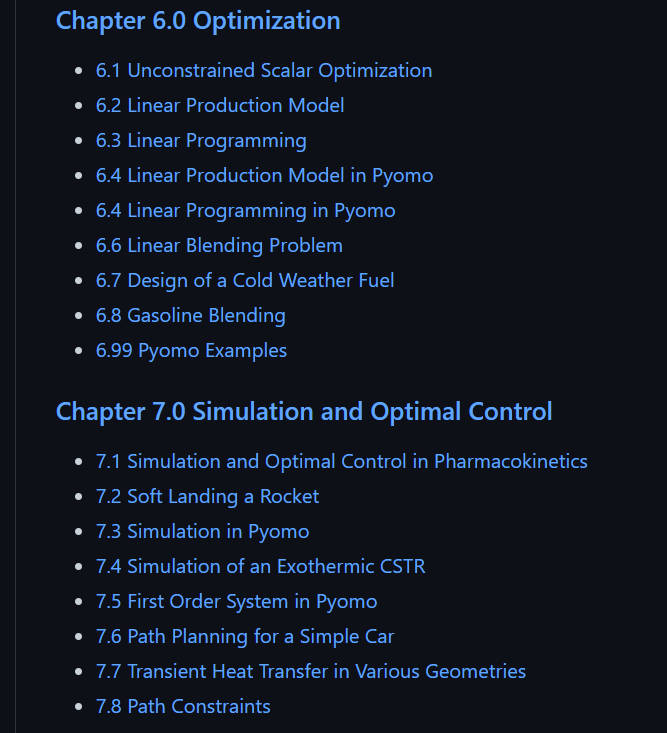
\includegraphics[width=0.8\columnwidth]{Pictures/Optimization_CBE.png}
	\caption[Short title]{CBE 30338 Chemical Process Control}
	\label{figure:CBE}
\end{figure}

\begin{figure}[H]
	\centering
	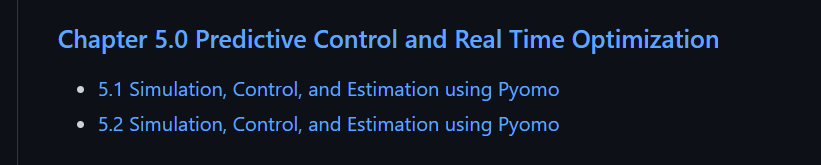
\includegraphics[width=0.8\columnwidth]{Pictures/Optimization_CBE_Lab.png}
	\caption[Short title]{CBE 32338 Process Control Laboratory}
	\label{figure:CBE_Lab}
\end{figure}

\newpage
	
	


%\bibliography{mybibliography}
\printbibliography[heading=bibintoc]

\end{document}
